\section{DataModel (Data Access Layer)}\label{sec:datamodel}

This is the library used by the \code{Server} and the \code{Scraper} to access
the database. This library is substantially an
\standout{ODM}\footnote{Object-Document Mapper.} that wraps and extends the
default mapper already available in the \mongodb{} Java Driver.

The Java classes are called POJOs\footnote{Plain Old Java Objects.}. These are
automatically translated into documents a vice versa by the \mongodb{} Java
Driver during the operations find, insert and replace. Unfortunately, the driver
is unable to keep track of the modifications made to the POJOs, so the library
we developed adds this functionality in order to allow to save the modifications
made to a POJO just with a simple call in the form \code{update(pojo)}.

The objective is to provide a generic and simple interface to the library's
user that works this way (pseudo-code):
\begin{verbatim}
manager = new Manager();
pojo = manager.find(/* filter query */);
/* work on the POJO by editing its fields or
 * call pojo.delete() to mark for deletion */
manager.save(pojo);
\end{verbatim}
The POJO instance will maintain a history of all modifications made in all its
fields and the \code{manager.save()} method will take care to do the
operation(s) needed to synchronize the document in the database with the POJO's
state.

The main classes in the library are the following:
\begin{itemize}
	\item[DBManager] It handles the connection with the database. It has
		various methods that allows to configure the connection options;
	\item[StorablePojo] This is the base class for all the POJOs that can be
		converted in document and stored in the database. This class
		maintains the state of the POJO, if it is marked for deletion or
		not and all the modifications done to all the fields;
	\item[PojoManager] A generic class to handle POJOs that should
		\standout{not} be saved in the database (supports only the find
		and aggregate operations). The user can extend this class in
		order to add more functionalities. All the find and aggregate
		methods return an instance of \code{PojoCursor} that wraps the
		\code{MongoCursor} class in order to properly handle the state
		of POJOs;
	\item[StorablePojoManager] Extends the \code{PojoManager} class to add
		support for the insert, updated, delete operations. All the
		operations return an instance of \code{StorablePojoCursor}.
\end{itemize}
The \code{StorablePojoManager} class may seem quite complex since it contains
some internal private classes and methods used to get the modifications made to
the POJOs through Java reflection and to generate the proper order of update
queries when a POJO need to be updated (\mongodb{}, in facts, does not allow to
make some update operations in the same query, such as a pull in a list while
updating a document in the same list).

Note that the POJOs can also be \emph{nested}: a POJO can contain other POJOs in
its fields (also inside a list). When the parent POJO is saved also all the
child POJOs are saved.

\begin{landscape}
	\begin{figure}[!h]
		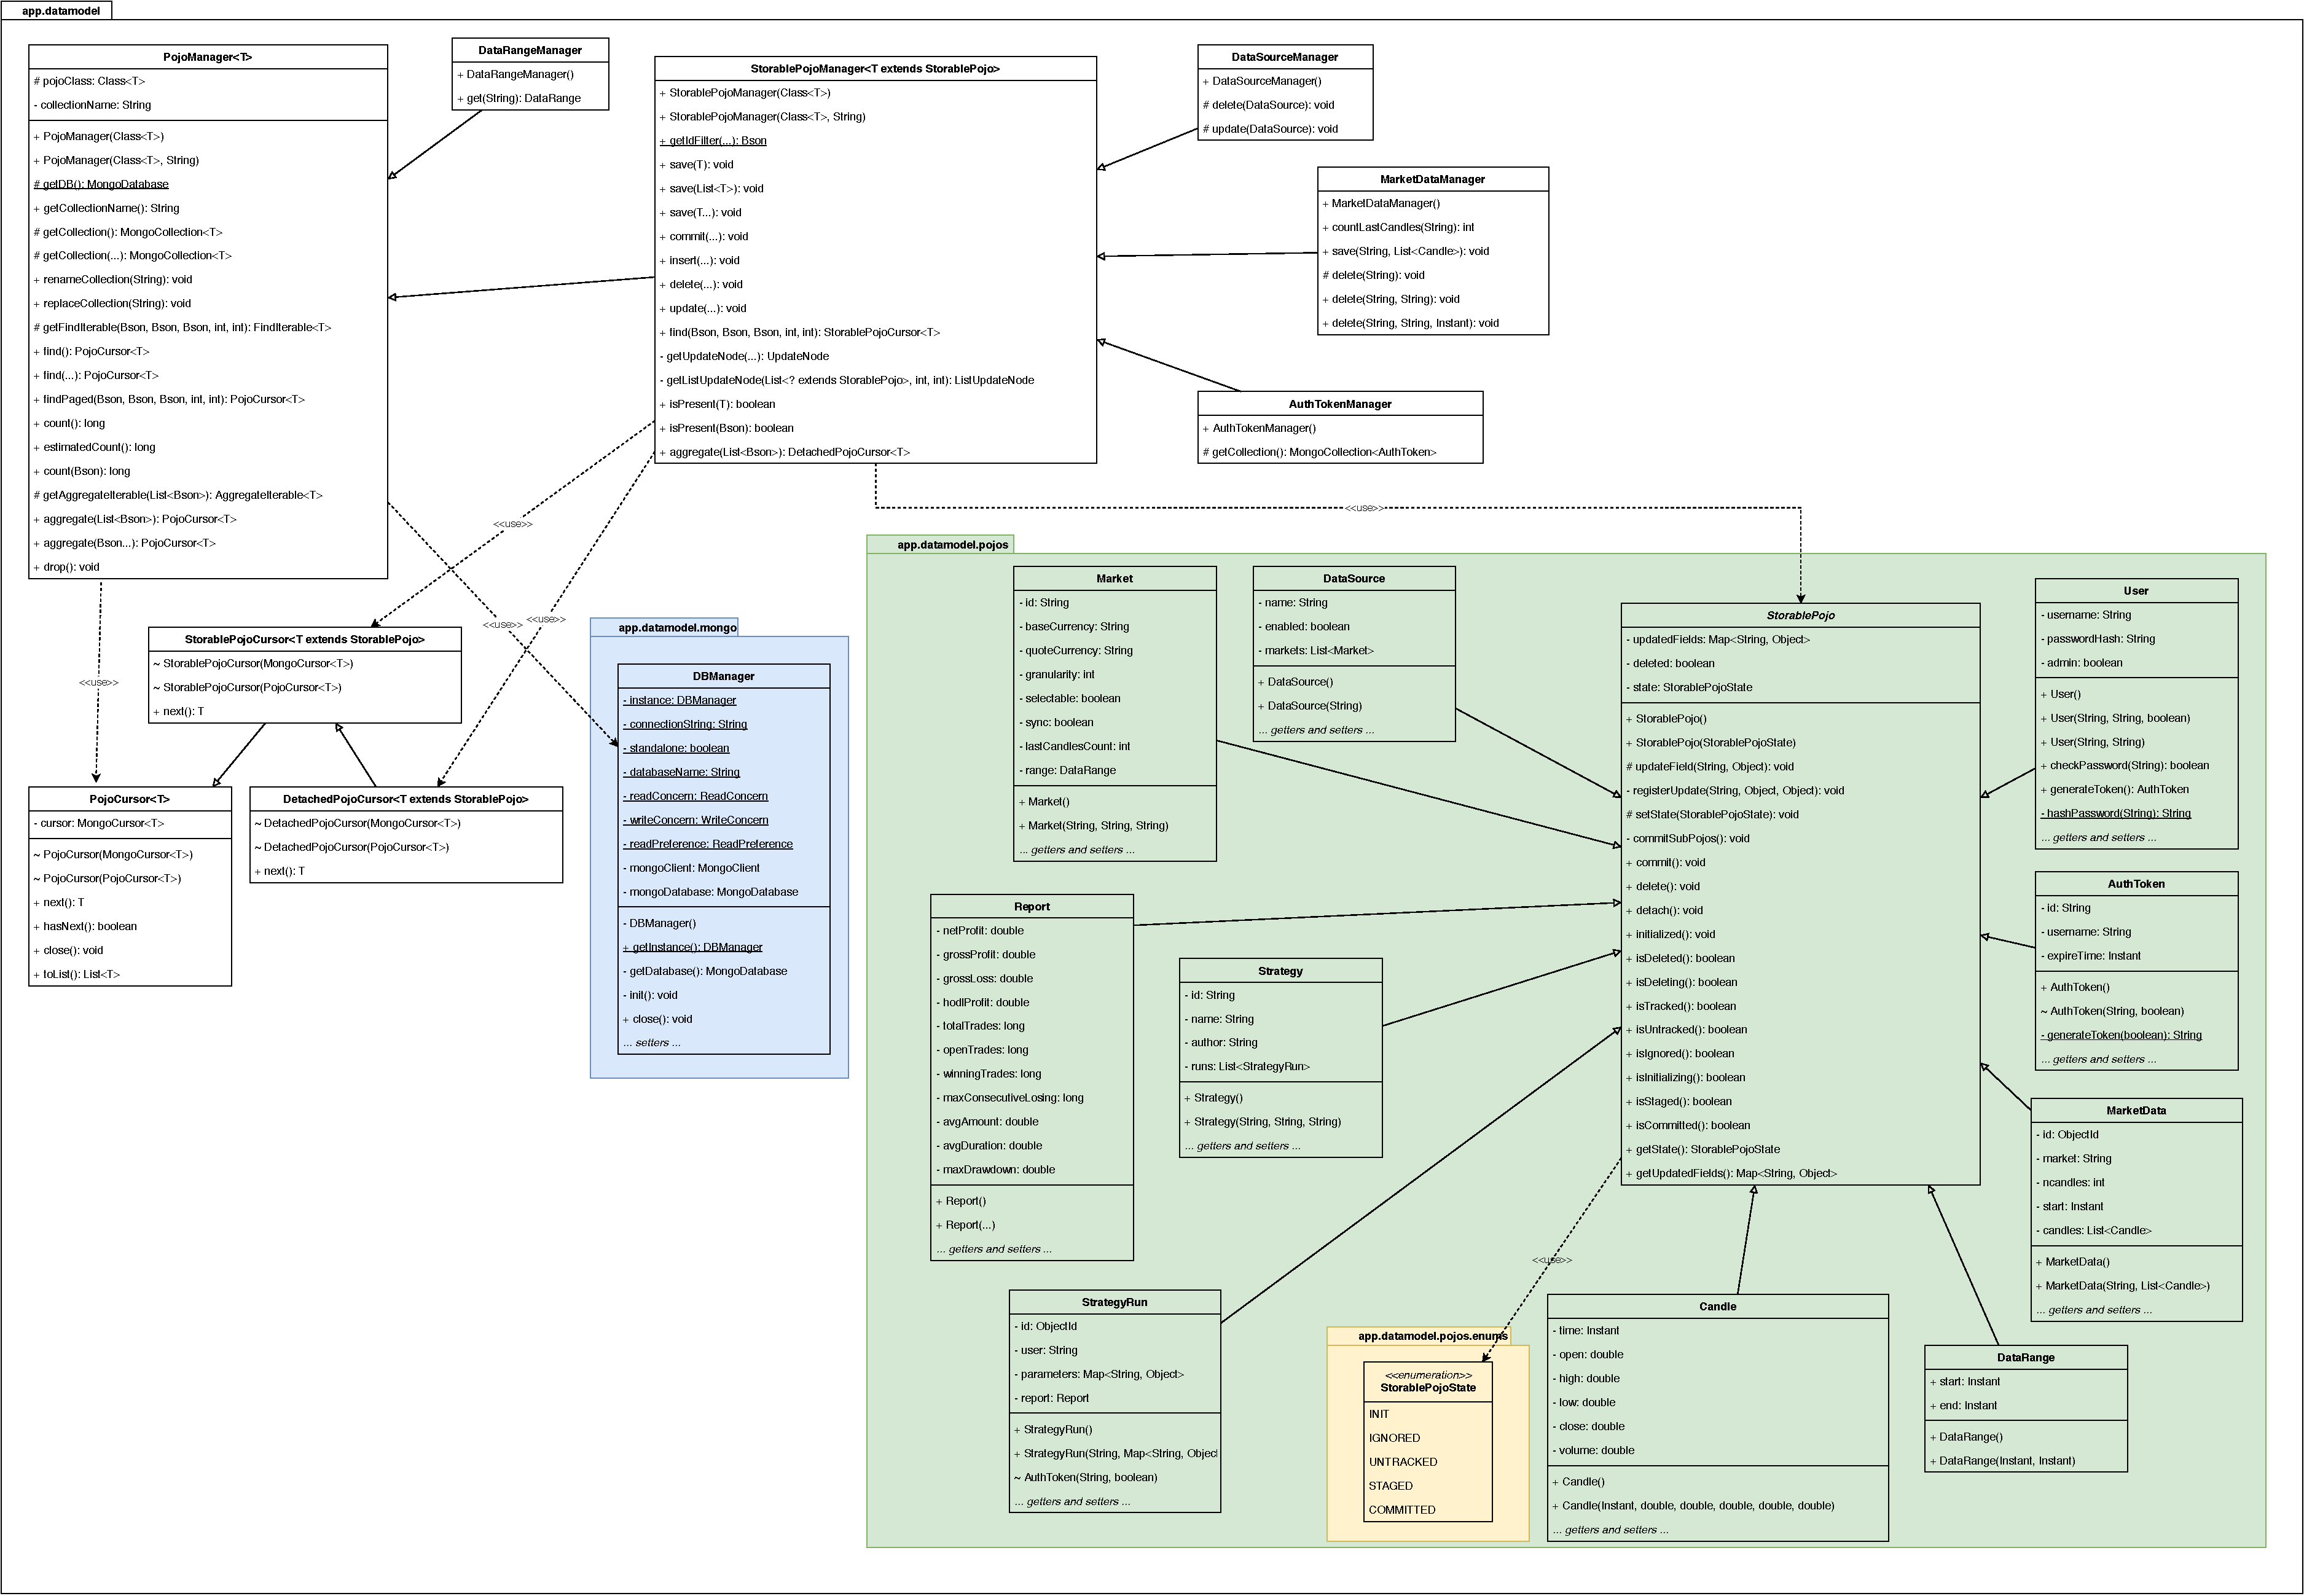
\includegraphics[width=0.8\paperheight]{module-datamodel}
		\caption*{\textbf{Figure~\ref{fig:datamodel}}}
		\captionlistentry{}\label{fig:datamodel}
	\end{figure}
\end{landscape}
